% ============================================================
%  CHAPITRE 4 — RELEASE 2 : IA, DEVOPS & MONITORING
% ============================================================
\chapter{Release 2 : Intelligence Artificielle, DevOps et Monitoring}

\vspace{-0.3cm}
\begin{tcolorbox}[colback=lightgray, colframe=primaryblue,
  title=\textbf{Plan}, fonttitle=\bfseries]
  \begin{enumerate}[leftmargin=*, label=\arabic*.]
    \item Sprint 4 --- Intelligence Artificielle (AI Assistant)
    \item Sprint 5 --- DevOps, Kubernetes \& Monitoring
  \end{enumerate}
\end{tcolorbox}

% ---------------------------------------------------------
\section*{Introduction}
% ---------------------------------------------------------

La deuxi\`eme release de SmartPM \'el\`eve la plateforme \`a un niveau
industriel en y int\'egrant deux dimensions compl\'ementaires et strat\'egiques.
D'une part, un assistant d'intelligence artificielle contextuel multi-LLM,
capable d'analyser les donn\'ees live des projets et de g\'en\'erer des rapports.
D'autre part, une infrastructure DevOps compl\`ete --- conteneurisation Docker,
orchestration Kubernetes, monitoring Prometheus/Grafana --- garantissant la haute
disponibilit\'e et la scalabilit\'e de la plateforme en production.

\vspace{0.3cm}

Pour chaque sprint, nous pr\'esentons les objectifs, le backlog, les diagrammes
UML (cas d'utilisation, classes, dynamiques) et les interfaces r\'ealis\'ees.

% ═══════════════════════════════════════════════════════════
\newpage
\section{Sprint 4 : Intelligence Artificielle --- AI Assistant}
\label{sec:s4}
% ═══════════════════════════════════════════════════════════

Ce quatri\`eme sprint a pour objectif de doter SmartPM d'un assistant
intelligent capable d'interagir en langage naturel avec les ing\'enieurs
a\'eronautiques et d'analyser les donn\'ees projets en temps r\'eel depuis
MongoDB Atlas.

\subsection{Objectifs du sprint 4}

\begin{itemize}
  \item D\'evelopper un chatbot contextuel aliment\'e par les donn\'ees live
        des projets SmartPM (MongoDB Atlas).
  \item Impl\'ementer une architecture \textbf{Multi-LLM avec fallback automatique} :
        Groq (priorit\'e 1) $\rightarrow$ Gemini (priorit\'e 2)
        $\rightarrow$ OpenRouter (priorit\'e 3).
  \item Cr\'eer un module de simulation de projets (pr\'ediction des risques
        de d\'erive et identification des membres surcharg\'es).
  \item Automatiser la g\'en\'eration de rapports d'avancement structur\'es.
  \item D\'evelopper le panneau \texttt{AiToolsPanel} regroupant tous les outils AI.
  \item Impl\'ementer le module de formations (Training) avec upload et
        indexation de documents de r\'ef\'erence DO-178C.
\end{itemize}

\subsection{Backlog du sprint 4}

\begin{table}[H]
\centering
\renewcommand{\arraystretch}{1.4}
\begin{tabularx}{\textwidth}{|c|X|c|c|}
\hline
\rowcolor{tablehead}
\textcolor{white}{\textbf{ID}} &
\textcolor{white}{\textbf{User Story}} &
\textcolor{white}{\textbf{Priorit\'e}} &
\textcolor{white}{\textbf{Charge (j)}} \\ \hline
US-4.1 & Utilisateur : interagir avec le chatbot AI (donn\'ees live MongoDB) & Haute & 4 \\ \hline
US-4.2 & Syst\`eme : bascule automatique Multi-LLM (Groq$\to$Gemini$\to$OpenRouter) & Haute & 3 \\ \hline
US-4.3 & Manager : simuler un projet (pr\'ediction d\'elais et risques) & Haute & 3 \\ \hline
US-4.4 & Manager : g\'en\'erer un rapport automatique via l'IA & Moyenne & 2 \\ \hline
US-4.5 & Utilisateur : acc\'eder au panneau AiToolsPanel & Moyenne & 2 \\ \hline
US-4.6 & Admin : uploader des documents de formation (Training) & Moyenne & 3 \\ \hline
\end{tabularx}
\caption{Backlog du Sprint 4 --- Intelligence Artificielle}
\label{tab:backlog_s4}
\end{table}

\subsection{Sp\'ecification des besoins fonctionnels}

\subsubsection{Architecture Multi-LLM de SmartPM}

L'une des innovations techniques majeures est l'architecture
\textbf{Multi-LLM avec fallback automatique}. Trois fournisseurs sont
utilis\'es de mani\`ere transparente :

\begin{itemize}
  \item \textbf{Groq} (priorit\'e 1) : fournisseur principal, mod\`ele
        \texttt{llama-3.3-70b-versatile}, latence inf\'erieure \`a 500ms
        pour le premier token.
  \item \textbf{Google Gemini} (priorit\'e 2) : mod\`ele
        \texttt{gemini-1.5-flash}, utilis\'e en cas de d\'epassement de
        quota ou d'indisponibilit\'e de Groq.
  \item \textbf{OpenRouter} (priorit\'e 3) : passerelle vers plusieurs
        mod\`eles (Claude, Mistral) pour garantir la continuit\'e de service.
\end{itemize}

\vspace{0.3cm}

La logique de fallback est impl\'ement\'ee dans \texttt{LlmRouterService}
du microservice FastAPI. En cas d'exception (\texttt{RateLimitError},
\texttt{APIConnectionError}), le service bascule automatiquement vers le
fournisseur suivant dans la cha\^ine de priorit\'e, sans interruption visible
par l'utilisateur.

\subsubsection{Contextualisation des requ\^etes AI}

Avant d'envoyer la requ\^ete au LLM, le backend NestJS enrichit le prompt
avec les informations live du projet : liste des projets actifs et leurs taux
d'avancement, t\^aches en retard, charge de travail de chaque membre,
statistiques des certifications, revues en attente depuis plus de 48 heures.
Ce contexte injecte dans le \textit{system prompt} permet \`a l'assistant
de r\'epondre \`a des questions comme \textit{<< Quels sont les projets
\`a risque cette semaine ? >>} avec des donn\'ees pr\'ecises et actualis\'ees.

\subsubsection{Diagramme de cas d'utilisation}

\begin{figure}[H]
  \centering
  \includegraphics[width=\textwidth]{figures/chapter4/sprint4/uc_sprint4.png}
  \caption{Diagramme de cas d'utilisation --- Sprint 4 (AI Assistant)}
  \label{fig:uc_s4}
\end{figure}

\subsection{Diagramme de classes du sprint 4}

\begin{figure}[H]
  \centering
  \includegraphics[width=\textwidth]{figures/chapter4/sprint4/class_sprint4.png}
  \caption{Diagramme de classes --- Sprint 4 (AI Assistant)}
  \label{fig:class_s4}
\end{figure}

\subsection{Diagrammes dynamiques du sprint 4}

\subsubsection{Diagramme de s\'equence --- Chatbot AI en streaming SSE}

Le diagramme~\ref{fig:seq_chat} d\'etaille le flux complet d'une interaction
avec le chatbot SmartPM. L'utilisation des \textit{Server-Sent Events} (SSE)
permet d'afficher la r\'eponse token par token, offrant une exp\'erience
utilisateur similaire \`a ChatGPT.

\vspace{0.3cm}

Le flux se d\'eroule en quatre \'etapes :
(1)~L'utilisateur envoie un message depuis \texttt{AiChatbotComponent} ;
(2)~le \texttt{AiIntegrationService} NestJS collecte le contexte live depuis
MongoDB Atlas ;
(3)~la requ\^ete enrichie est transmise au microservice FastAPI qui appelle
le LLM s\'electionn\'e ;
(4)~les tokens sont relay\'es en streaming SSE vers le client Angular.

\begin{figure}[H]
  \centering
  \includegraphics[width=\textwidth]{figures/chapter4/sprint4/seq_chatbot.png}
  \caption{Diagramme de s\'equence --- Chatbot AI avec streaming SSE}
  \label{fig:seq_chat}
\end{figure}

\subsubsection{Diagramme d'activit\'e --- Logique de fallback Multi-LLM}

\begin{figure}[H]
  \centering
  \includegraphics[width=\textwidth]{figures/chapter4/sprint4/activity_llm_fallback.png}
  \caption{Diagramme d'activit\'e --- Strat\'egie Multi-LLM avec fallback}
  \label{fig:act_llm}
\end{figure}

\subsection{R\'ealisation du sprint 4}

Le module \texttt{AiIntegrationModule} NestJS joue le r\^ole de passerelle
entre Angular et le microservice FastAPI. Le microservice IA est d\'evelopp\'e
en \textbf{Python 3.11} avec \textbf{FastAPI} et la biblioth\`eque
\textbf{LangChain} pour abstraire les appels aux diff\'erents LLMs.
Il expose trois endpoints : \texttt{POST /chat/stream} (chatbot streaming),
\texttt{POST /simulate} (simulation projet) et \texttt{POST /report}
(g\'en\'eration rapport).

\begin{figure}[H]
  \centering
  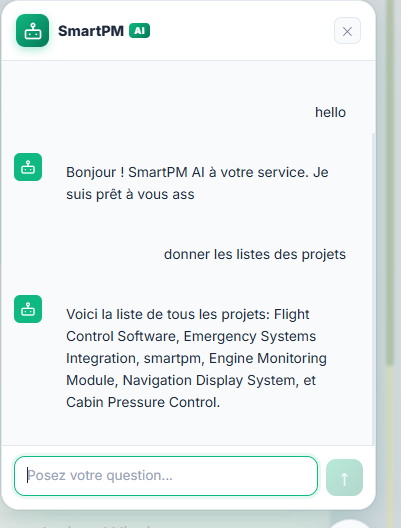
\includegraphics[width=\textwidth]{images/screen_chatbot.png}
  \caption{Interface du chatbot AI contextuel de SmartPM}
  \label{fig:scr_chat}
\end{figure}

\begin{figure}[H]
  \centering
  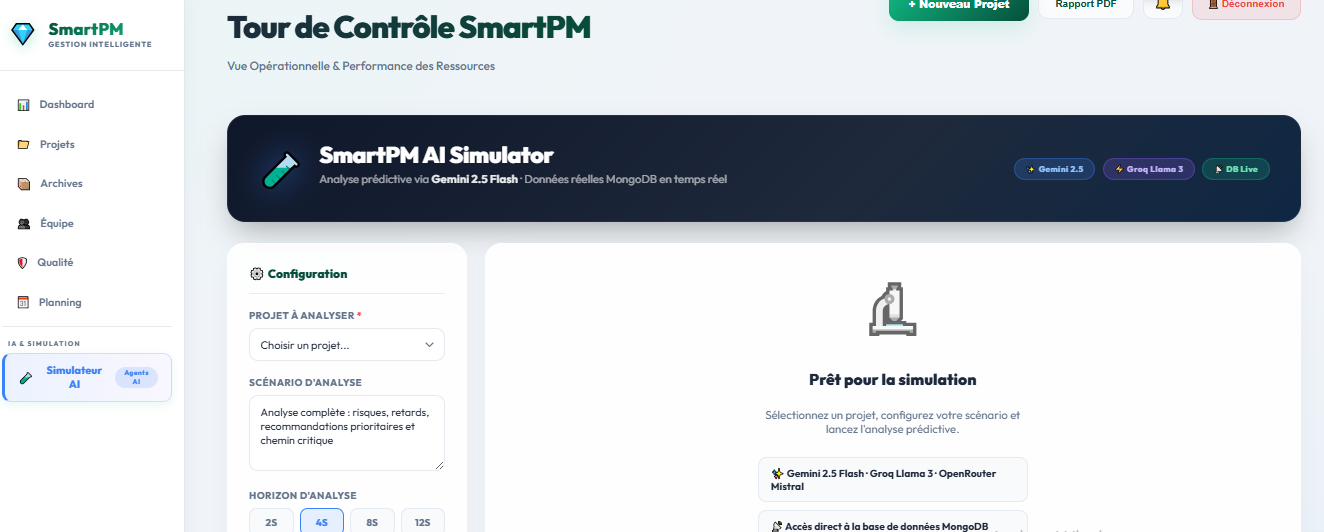
\includegraphics[width=\textwidth]{images/screen_ai_tools.png}
  \caption{AiToolsPanel --- Panneau centralis\'e des outils IA}
  \label{fig:scr_tools}
\end{figure}

\begin{figure}[H]
  \centering
  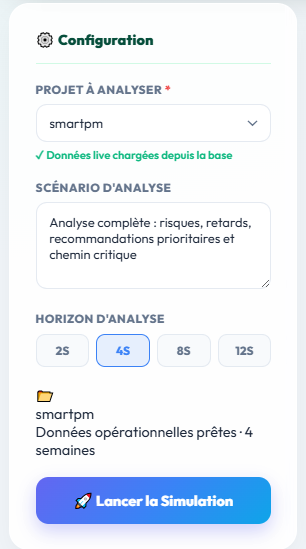
\includegraphics[width=\textwidth]{images/screen_simulation.png}
  \caption{Module de simulation --- Pr\'ediction des risques par l'IA}
  \label{fig:scr_sim}
\end{figure}

\begin{figure}[H]
  \centering
  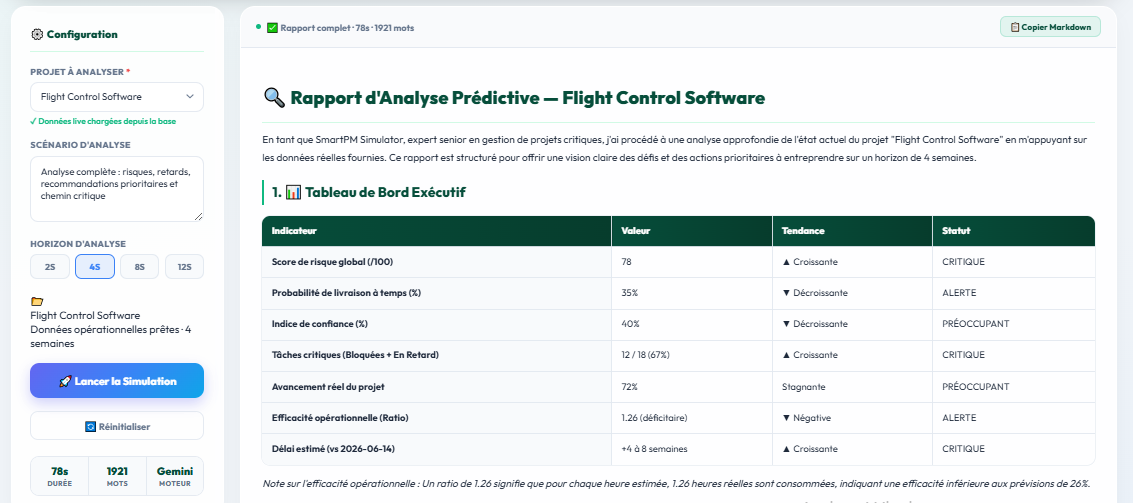
\includegraphics[width=\textwidth]{images/screen_report.png}
  \caption{G\'en\'eration automatique de rapport d'avancement via l'IA}
  \label{fig:scr_report}
\end{figure}

\begin{figure}[H]
  \centering
  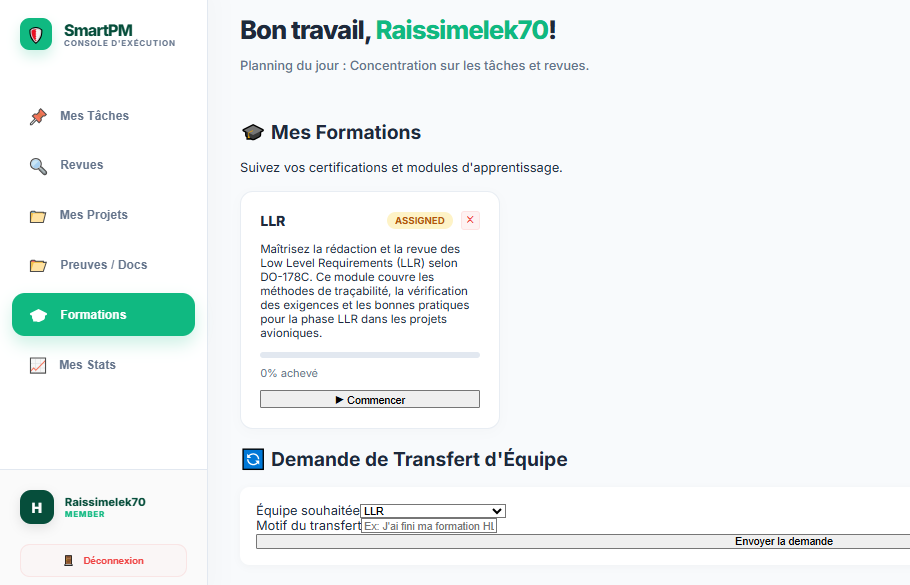
\includegraphics[width=\textwidth]{images/screen_training.png}
  \caption{Module Training --- Gestion des documents de r\'ef\'erence DO-178C}
  \label{fig:scr_train}
\end{figure}

% ═══════════════════════════════════════════════════════════
\newpage
\section{Sprint 5 : DevOps, Kubernetes \& Monitoring}
\label{sec:s5}
% ═══════════════════════════════════════════════════════════

Ce cinqui\`eme et dernier sprint industrialise le d\'eploiement de SmartPM
en le dotant d'une infrastructure de production robuste, automatis\'ee et
observable. Il s'articule autour de trois axes : \textbf{conteneurisation}
Docker, \textbf{orchestration} Kubernetes et \textbf{monitoring}
Prometheus/Grafana.

\subsection{Objectifs du sprint 5}

\begin{itemize}
  \item Cr\'eer des \texttt{Dockerfile} optimis\'es (multi-stage) pour les
        trois services : frontend Angular, backend NestJS, service AI FastAPI.
  \item \'Ecrire les manifestes Kubernetes YAML pour les six deployments.
  \item Configurer Prometheus (endpoint \texttt{/metrics}) et Grafana
        (dashboards pr\'econfig\'ur\'es).
  \item S\'ecuriser le backend avec Helmet, ThrottlerGuard (100~req/min/IP)
        et une politique CORS stricte.
  \item Impl\'ementer le \texttt{BackupReplicationService} MongoDB Atlas.
  \item Automatiser le d\'eploiement via le script \texttt{start-devops.bat}.
\end{itemize}

\subsection{Backlog du sprint 5}

\begin{table}[H]
\centering
\renewcommand{\arraystretch}{1.4}
\begin{tabularx}{\textwidth}{|c|X|c|c|}
\hline
\rowcolor{tablehead}
\textcolor{white}{\textbf{ID}} &
\textcolor{white}{\textbf{User Story}} &
\textcolor{white}{\textbf{Priorit\'e}} &
\textcolor{white}{\textbf{Charge (j)}} \\ \hline
US-5.1 & Dockerfile optimis\'e pour les 3 services (frontend, backend, AI) & Haute & 2 \\ \hline
US-5.2 & Manifestes K8s : 6 Deployments + Services (NodePort) & Haute & 3 \\ \hline
US-5.3 & Prometheus : collecte m\'etriques API NestJS (\texttt{/metrics}) & Haute & 2 \\ \hline
US-5.4 & Grafana : dashboards m\'etriques API et \'etat des pods & Haute & 2 \\ \hline
US-5.5 & S\'ecurit\'e backend : Helmet + ThrottlerGuard + CORS strict & Haute & 1 \\ \hline
US-5.6 & BackupReplicationService MongoDB Atlas & Moyenne & 2 \\ \hline
US-5.7 & Script CI/CD automatis\'e : start-devops.bat & Moyenne & 1 \\ \hline
\end{tabularx}
\caption{Backlog du Sprint 5 --- DevOps, Kubernetes \& Monitoring}
\label{tab:backlog_s5}
\end{table}

\subsection{Sp\'ecification des besoins fonctionnels}

\subsubsection{Diagramme de cas d'utilisation}

\begin{figure}[H]
  \centering
  \includegraphics[width=\textwidth]{figures/chapter4/sprint5/uc_sprint5.png}
  \caption{Diagramme de cas d'utilisation --- Sprint 5 (DevOps \& Monitoring)}
  \label{fig:uc_s5}
\end{figure}

\subsection{Diagramme de classes du sprint 5}

L'infrastructure DevOps ne g\'en\`ere pas d'entit\'es de donn\'ees \`a
proprement parler. Les principaux artefacts sont les configurations
Kubernetes (Deployment, Service, ConfigMap, PersistentVolumeClaim) et les
tableaux de bord Grafana. Le tableau~\ref{tab:k8s_pods} r\'ecapitule les
composants d\'eploy\'es.

\begin{table}[H]
\centering
\renewcommand{\arraystretch}{1.4}
\begin{tabularx}{\textwidth}{|l|l|c|c|}
\hline
\rowcolor{tablehead}
\textcolor{white}{\textbf{Deployment}} &
\textcolor{white}{\textbf{Image Docker}} &
\textcolor{white}{\textbf{Replicas}} &
\textcolor{white}{\textbf{NodePort}} \\ \hline
frontend   & smartpm/frontend:latest   & 2 & 30080 \\ \hline
backend    & smartpm/backend:latest    & 2 & 30000 \\ \hline
ai-service & smartpm/ai:latest         & 1 & 30800 \\ \hline
prometheus & prom/prometheus:latest    & 1 & 30090 \\ \hline
grafana    & grafana/grafana:latest    & 1 & 30300 \\ \hline
mongo      & MongoDB Atlas (Cloud)     & --- & --- \\ \hline
\end{tabularx}
\caption{R\'ecapitulatif des Deployments Kubernetes de SmartPM}
\label{tab:k8s_pods}
\end{table}

\subsection{Diagrammes dynamiques du sprint 5}

\subsubsection{Architecture de d\'eploiement Kubernetes}

\begin{figure}[H]
  \centering
  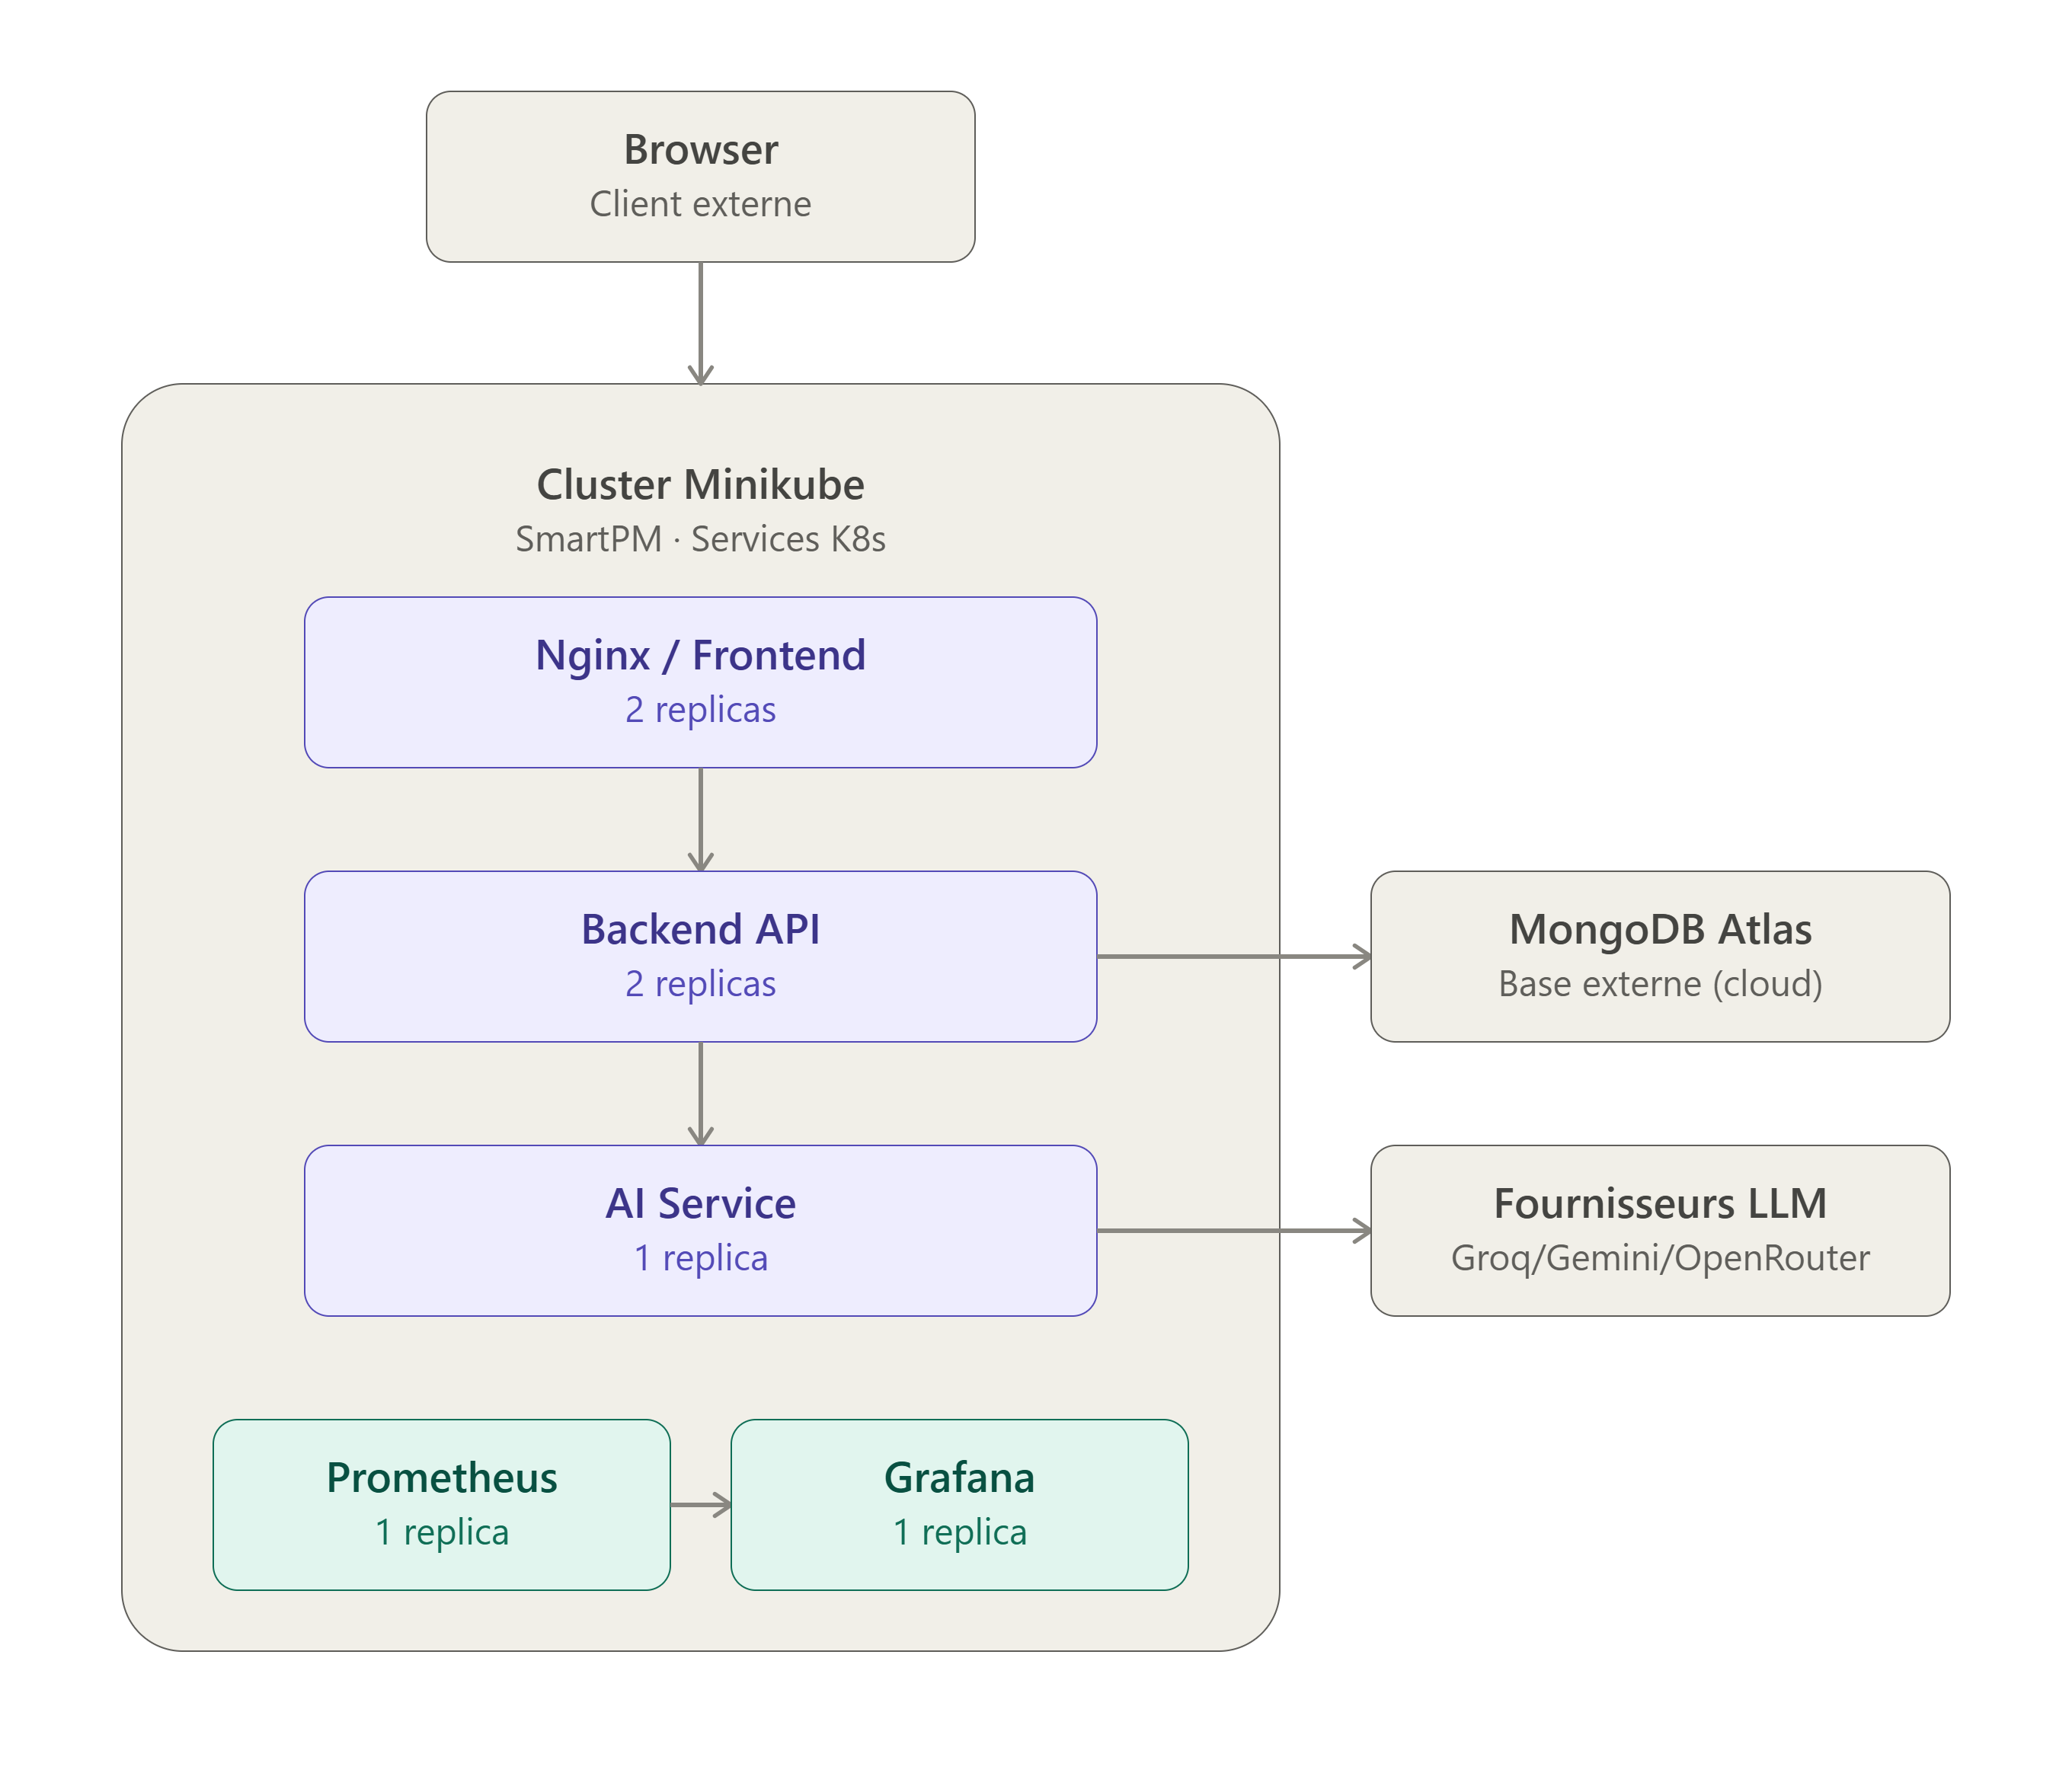
\includegraphics[width=\textwidth]{images/arch_k8s.png}
  \caption{Architecture de d\'eploiement Kubernetes de SmartPM}
  \label{fig:arch_k8s}
\end{figure}

\subsubsection{Diagramme de s\'equence --- Pipeline CI/CD}

Le script \texttt{start-devops.bat} automatise six \'etapes s\'equentielles :
(1)~v\'erification Minikube, (2)~\texttt{docker build} des trois images,
(3)~\texttt{minikube image load}, (4)~\texttt{kubectl apply -f k8s/},
(5)~attente que tous les pods soient \texttt{Running}, (6)~affichage
des URLs d'acc\`es.

\begin{figure}[H]
  \centering
  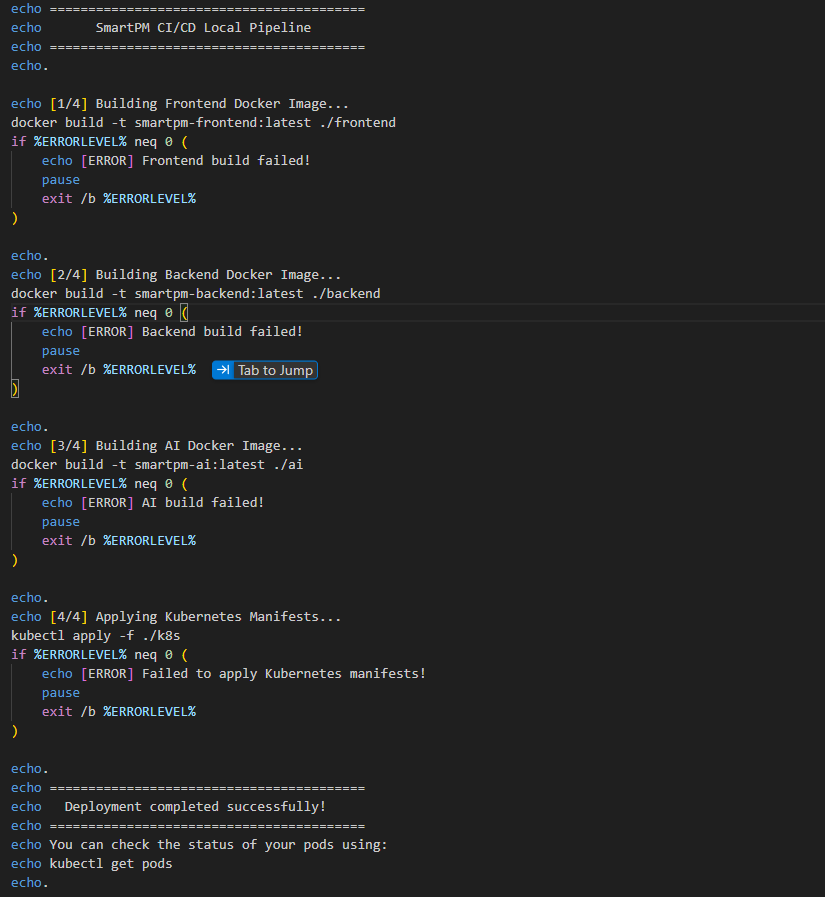
\includegraphics[width=\textwidth]{images/pipeline_cicd.png}
  \caption{Pipeline CI/CD automatis\'e --- \texttt{start-devops.bat}}
  \label{fig:pipeline}
\end{figure}

\subsection{R\'ealisation du sprint 5}

\subsubsection{Conteneurisation Docker}

Les trois services sont conteneuris\'es avec des Dockerfiles optimis\'es :
\textbf{Frontend} en build multi-stage (\texttt{node:20-alpine} pour la
compilation Angular + \texttt{nginx:alpine} pour le service, image finale
$<$50\,MB) ;
\textbf{Backend NestJS} bas\'e sur \texttt{node:20-alpine} avec
\texttt{npm ci --only=production} ;
\textbf{Service AI} bas\'e sur \texttt{python:3.11-slim} avec
\texttt{uvicorn main:app --host 0.0.0.0 --port 8000}.

\subsubsection{S\'ecurisation multi-couches du backend}

Trois couches de s\'ecurit\'e compl\'ementaires ont \'et\'e ajout\'ees :
\textbf{Helmet} (en-t\^etes HTTP : \texttt{X-Frame-Options: DENY},
\texttt{Content-Security-Policy}, \texttt{Strict-Transport-Security}),
\textbf{ThrottlerGuard} (100 requ\^etes/minute/IP, anti-DDoS et
anti-brute-force) et \textbf{CORS strict} (origines autoris\'ees via
\texttt{ALLOWED\_ORIGINS}).

\subsubsection{Monitoring Prometheus \& Grafana}

Le module \texttt{@willsoto/nestjs-prometheus} expose l'endpoint
\texttt{GET /metrics} en format Prometheus, collectant :
\texttt{http\_request\_duration\_seconds} (histogramme de latence par route),
\texttt{http\_requests\_total} (compteur par statut HTTP),
\texttt{nodejs\_heap\_size\_used\_bytes} (m\'emoire heap) et
\texttt{process\_cpu\_seconds\_total} (CPU).

\vspace{0.3cm}

Deux dashboards Grafana sont pr\'econfig\'ur\'es via ConfigMap Kubernetes :
\textbf{Dashboard API SmartPM} (requ\^etes/minute, latence P95, taux d'erreurs)
et \textbf{Dashboard Infrastructure} (\'etat des pods, CPU, m\'emoire).

\subsubsection{Interfaces r\'ealis\'ees}

\begin{figure}[H]
  \centering
  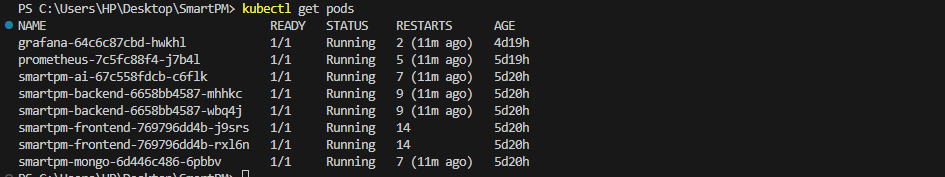
\includegraphics[width=\textwidth]{images/screen_kubectl_pods.png}
  \caption{\'Etat des pods Kubernetes --- \texttt{kubectl get pods}}
  \label{fig:scr_k8s}
\end{figure}

\begin{figure}[H]
  \centering
  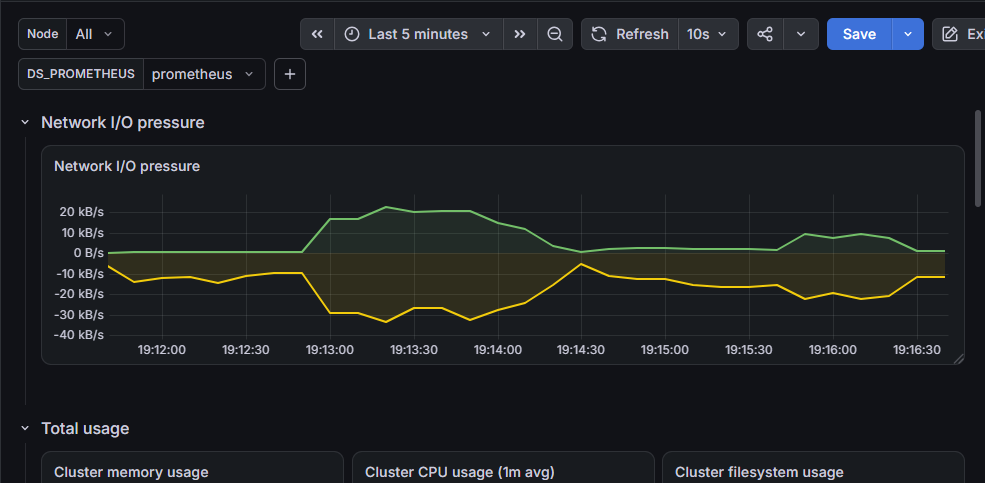
\includegraphics[width=\textwidth]{images/screen_grafana.png}
  \caption{Dashboard Grafana --- M\'etriques API de SmartPM}
  \label{fig:scr_grafana}
\end{figure}

\begin{figure}[H]
  \centering
  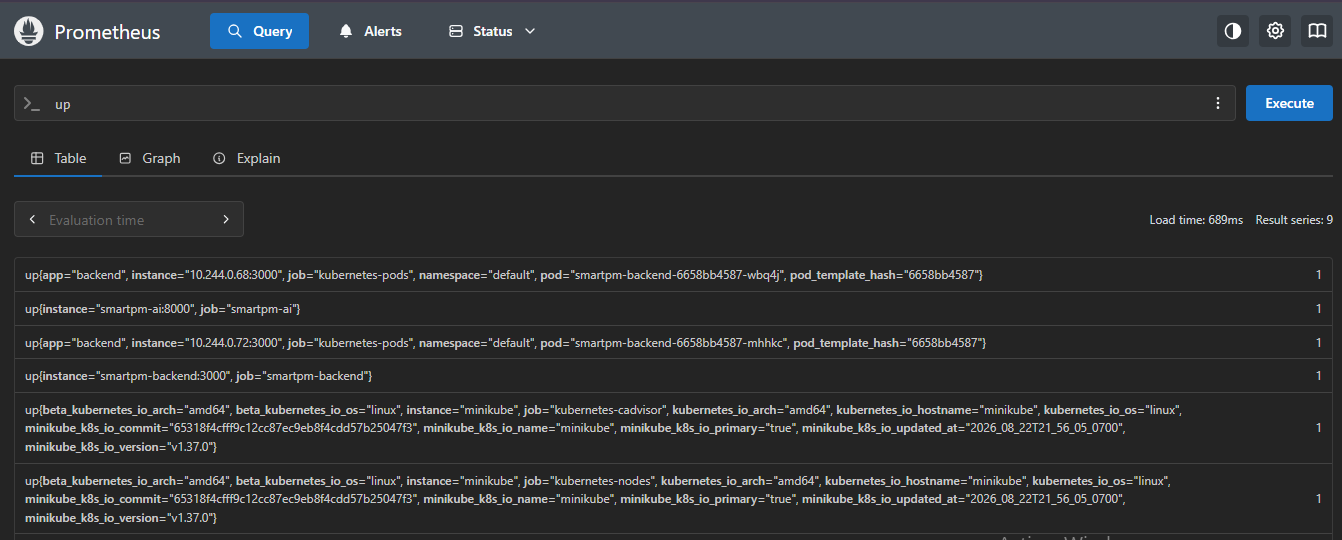
\includegraphics[width=\textwidth]{images/screen_prometheus.png}
  \caption{Interface Prometheus --- Supervision des m\'etriques}
  \label{fig:scr_prom}
\end{figure}

\begin{figure}[H]
  \centering
  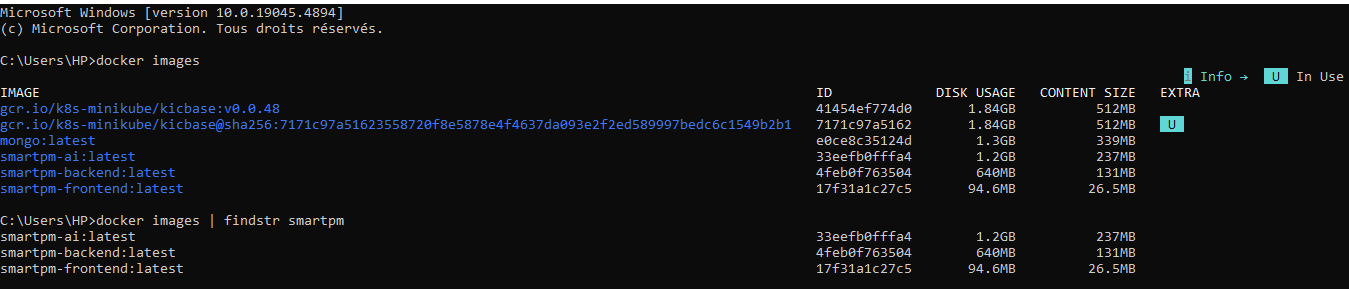
\includegraphics[width=\textwidth]{images/screen_docker_images.png}
  \caption{Images Docker construites pour SmartPM}
  \label{fig:scr_docker}
\end{figure}

% ---------------------------------------------------------
\section*{Conclusion}
% ---------------------------------------------------------

La deuxi\`eme release marque l'aboutissement technique du projet SmartPM.
L'int\'egration d'un assistant AI contextuel multi-LLM avec streaming SSE
apporte une valeur ajout\'ee significative et diff\'erenciante pour les
ing\'enieurs a\'eronautiques, en leur offrant une assistance intelligente
nourrie des donn\'ees r\'eelles de leurs projets.

\vspace{0.3cm}

L'infrastructure Kubernetes d\'eploy\'ee garantit la scalabilit\'e, la
r\'esilience et la tra\c{c}abilit\'e compl\`ete des services en production.
Le monitoring Prometheus/Grafana assure une observabilit\'e en temps r\'eel,
indispensable dans un contexte industriel o\`u la disponibilit\'e est critique.

\vspace{0.3cm}

La plateforme SmartPM est d\'esormais op\'erationnelle, s\'ecuris\'ee et
monitor\'ee, pr\^ete \`a \'evoluer vers une int\'egration compl\`ete dans
les cha\^ines d'outillage de certification DO-178C de niveau DAL-A.
